    %!TEX encoding = UTF-8 Unicode 
\documentclass[usenames,dvipsnames]{beamer}

    \usetheme{metropolis}

   \usecolortheme{seahorse}
   
        \usepackage{pgfpages}
\usepackage{CJKutf8} 
\usepackage{tcolorbox}
\usepackage[textfont={small}]{caption}

    \setbeamercovered{invisible}
    \usepackage{tikz}   
    \usetikzlibrary{shapes,arrows}
\usepackage{graphicx}% http://ctan.org/pkg/graphicx
\usepackage{booktabs}
    \usepackage{framed, color}
    \definecolor{shadecolor}{rgb}{1, 0.8, 0.3}
    % To remove the navigation symbols from
    % the bottom of slides%
 %\setbeameroption{show notes on second screen}
%\setbeameroption{show only notes}
    \setbeamertemplate{navigation symbols}{}
    %
  \setbeamercolor{section in head/foot}{fg=black, bg=structure.fg!20!white}

\usepackage[natbibapa]{apacite}
\bibliographystyle{apacite}
\bibpunct{(}{)}{;}{a}{}{,}

\usetikzlibrary{calc}


\tikzstyle{decision} = [diamond, draw, fill=blue!20, 
    text width=4.5em, text badly centered, node distance=3cm, inner sep=0pt]
\tikzstyle{block} = [rectangle, draw, fill=blue!20, 
    text width=6em, text centered, rounded corners, minimum height=4em]
\tikzstyle{line} = [draw, -latex']
\tikzstyle{cloud} = [draw, ellipse,fill=red!20, node distance=3cm,
    minimum height=2em]

\newcommand{\tikzmark}[1]{\tikz[overlay,remember picture] \node (#1) {};}
\newcommand{\DrawBox}[1][]{%
    \tikz[overlay,remember picture]{
    \draw[red,#1]
      ($(left)+(-0.2em,0.9em)$) rectangle
      ($(right)+(0.2em,-0.3em)$);}
}

\newenvironment{variableblock}[3]{%
  \setbeamercolor{block body}{#2}
  \setbeamercolor{block title}{#3}
  \begin{block}{#1}}{\end{block}}

\makeatletter
\setbeamertemplate{footline}
{
  \leavevmode%
  \hbox{%
  \begin{beamercolorbox}[wd=1\paperwidth,ht=2.25ex,dp=1ex,center]{author in head/foot}%
    \usebeamerfont{author in head/foot}%
    \insertsectionnavigationhorizontal{0.8\paperwidth }{}{}%
     \insertframenumber /  \inserttotalframenumber
 \end{beamercolorbox}}%
 % \begin{beamercolorbox}[wd=.3\paperwidth,ht=2.25ex,dp=1ex,right]{date in head/foot}%
   % \usebeamerfont{date in head/foot}\insertshortdate{}\hspace*{2em}
  \hspace*{2ex} 
  %\end{beamercolorbox}}%
  \vskip0pt%
}


\usepackage{graphicx}
\usepackage[caption=false]{subfig}
\usepackage{multicol}
\usepackage{color, colortbl}
\definecolor{Gray}{gray}{0.9}

%\definecolor{white}{white}{0.9}

%\setbeamercovered{white}
    %\usepackage{bm} % For typesetting bold math (not \mathbold)
    %\logo{\includegraphics[height=0.6cm]{yourlogo.eps}}
\title{Does providing corruption information reduce vote share? A meta-analysis}
\date{\today} 
\author{Trevor Incerti}
\institute{Yale University}

\begin{document}
\maketitle

%%%%%%%%%%%%%%%%%%%%%%%%%%%%%%%%%%%

\section{Introduction}

\begin{frame}
\frametitle{Research Question}
Do voters in democratic countries hold politicians accountable for corruption?
\pause
\begin{itemize}
\item Key question of electoral accountability. 
\pause
\item Recent ARPS review (\citet{de2017electoral}): ``Empirical evidence to date is \textcolor{Cerulean}{mixed}, and it often suggests that the electoral punishment of corruption is rather mild.'' 
\pause
\item Is evidence actually mixed? What have we learned from a recent explosion of experimental research on this subject?
\end{itemize}
\end{frame}

%%%%%%%%%%%%%%%%%%%%%%%%%%%%%%%%%%%

\section{Methods}

\begin{frame}
\frametitle{Meta-Analysis}
Meta-analysis of all \textcolor{Cerulean}{experimental} studies conducted to date. 
\pause
\begin{itemize}
\item \textcolor{Cerulean}{Treatment}: corruption information provision. 
\pause
\item \textcolor{Cerulean}{Outcome}: (incumbent) vote-share.
\pause
\item Random assignment of information regarding
incumbent corruption, followed by measurement of voting outcomes.
\pause
\item Includes both \textcolor{Cerulean}{published articles and working papers}.
\pause
\item Excludes experiments that inform all respondents that the politician is corrupt.
\begin{itemize}
\item E.g. Compare one type of information provision (e.g. source) to another.
\end{itemize}
\end{itemize}
\end{frame}

%%%%%%%%%%%%%%%%%%%%%%%%%%%%%%%%%%%

\begin{frame}
\frametitle{Analytical details}
\begin{itemize}
\item Where there are multiple corruption treatments (e.g. varying source of information), I replicate the studies and code corruption as a binary treatment (0 = clean, 1 = corrupt).
\pause
\item Studies that use non-binary vote choices are rescaled into a binary vote choice.
\pause
\item Point estimates, standard errors and/or confidence intervals are not always explicitly reported (4 cases). In these cases standard errors are estimated by digitally measuring coefficient plots.
\end{itemize}

\end{frame}

%%%%%%%%%%%%%%%%%%%%%%%%%%%%%%%%%%%

\section{Results}

\begin{frame}
\frametitle{Results: Field Experiments}

\only<1>{
\begin{figure}
\hspace*{-11mm}
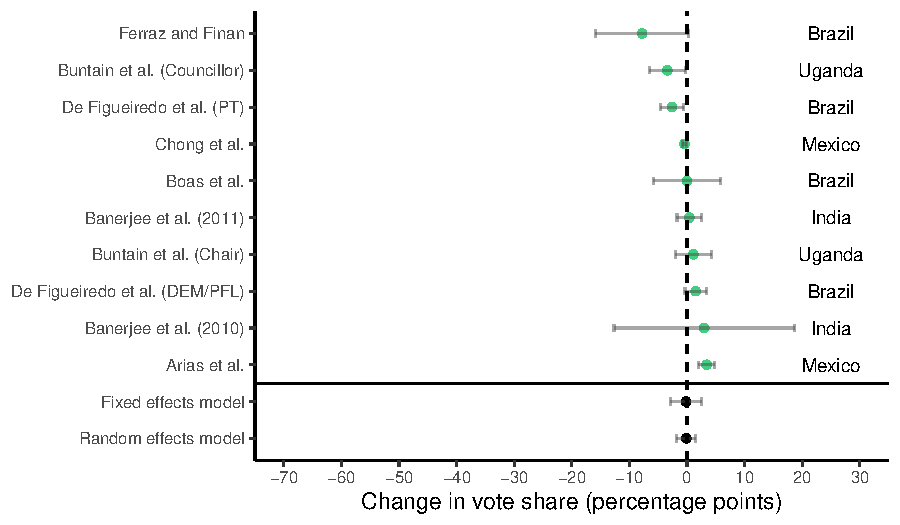
\includegraphics[scale=0.83]{../figs/field.pdf}
\end{figure}
}

\end{frame}

%%%%%%%%%%%%%%%%%%%%%%%%%%%%%%%%%%%

\begin{frame}
\frametitle{Results: Survey Experiments}

\only<1>{
\begin{figure}
\vspace*{-1cm}
\hspace*{-11mm}
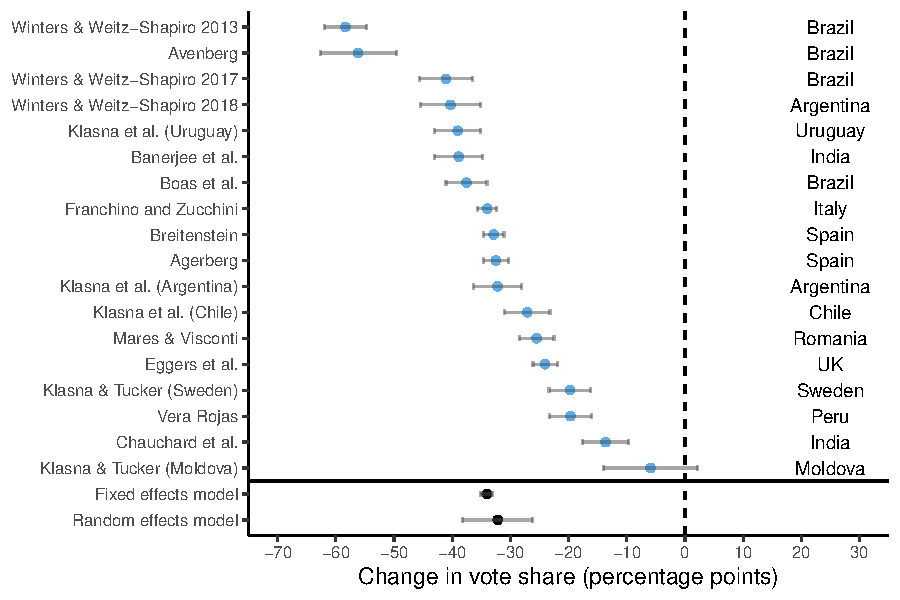
\includegraphics[scale=0.83]{../figs/survey.pdf}
\end{figure}
}

\end{frame}

%%%%%%%%%%%%%%%%%%%%%%%%%%%%%%%%%%%

\begin{frame}
\frametitle{Results}
\begin{itemize}
\item Survey experiments overestimate the ATE of providing corruption information to voters relative to field experiments.
\pause
\begin{itemize}
\item Corrupt candidates punished by approximately \textcolor{Cerulean}{zero percentage points} in field experiments.
\pause
\item Corrupt candidates punished by respondents by between \textcolor{Cerulean}{33 percentage points} (random effects) and \textcolor{Cerulean}{35 percentage points} (fixed effects) in survey experiments.
\pause
\item 70\% of the total heterogeneity across studies can be accounted for by including a dummy variable for type of experiment.
\pause
\item Point estimate of this dummy variable (0 = survey, 1 = field) is equal to 0.32 (significant at 1\% level), while the overall estimate across studies is -.33. 
\begin{itemize}
\item Mixed effects meta-analysis with moderator. 
\end{itemize}
\end{itemize}
\end{itemize}
\end{frame}

%%%%%%%%%%%%%%%%%%%%%%%%%%%%%%%%%%%
\section{Discussion}

\begin{frame}
\frametitle{Discussion}
What might account for this discrepancy?
\pause
\begin{itemize}
\item Publication bias and/or p-hacking
\pause
\item Social desirability bias
\pause
\item Lack of complexity in survey experiments.
\pause
\item Analyzing/interpreting results of survey experiments incorrectly. 
\end{itemize}

\end{frame}

%%%%%%%%%%%%%%%%%%%%%%%%%%%%%%%%%%%

\begin{frame}
\frametitle{Publication bias and p-hacking}
\textcolor{Cerulean}{Little evidence of publication bias} within survey experiments:
\pause
\begin{itemize}
\item P-curve - virtually all results significant at 1\% level (not clustered around 0.05).
\pause
\item Tests for funnel plot asymmetry. 
\end{itemize}
\pause
Unclear with field experiments
\begin{itemize}
\item Five of eight papers published. Three unpublished papers all have null findings. 
\pause
\item Not enough data for formal tests. 
\end{itemize}
\pause
But, \textcolor{Cerulean}{differences in experimental design} likely account for the difference in the magnitude of treatment effects.

\end{frame}

%%%%%%%%%%%%%%%%%%%%%%%%%%%%%%%%%%%
\begin{frame}
\frametitle{Social desirability bias}
\begin{itemize}
\pause
\item Anti-corruption norms exist in most countries.
\begin{itemize}
\pause
\item No costs to selecting the socially desirable option in hypothetical vignette. 
\pause
\item In actual election voters may discount information, or have strong material/ideological incentives to stick with candidate.
\end{itemize}
\pause
\item How to overcome social desirability bias in survey experiments?
\begin{itemize}
\pause
\item Perform experiments during \textcolor{Cerulean}{actual elections} using real candidates.
\pause
\item Use \textcolor{Cerulean}{list experiments}, which have been shown to make a difference in admission to vote-buying \citep{gonzalez2012vote}.
\end{itemize}
\end{itemize}

\end{frame}

%%%%%%%%%%%%%%%%%%%%%%%%%%%%%%%%%%%
\begin{frame}
\frametitle{Survey complexity and conjoint experiments}
Randomizing more candidate characteristics may more adequately capture moderating factors and reduce social desirability bias.
\begin{itemize}
\pause
\item But, traditional method of analysis (comparing magnitudes of individual average marginal component effects) may be misleading. 
\end{itemize}

\end{frame}

%%%%%%%%%%%%%%%%%%%%%%%%%%%%%%%%%%%
\begin{frame}
\frametitle{Survey complexity and conjoint experiments}

\begin{figure}[!hb]
\hspace*{-11mm}
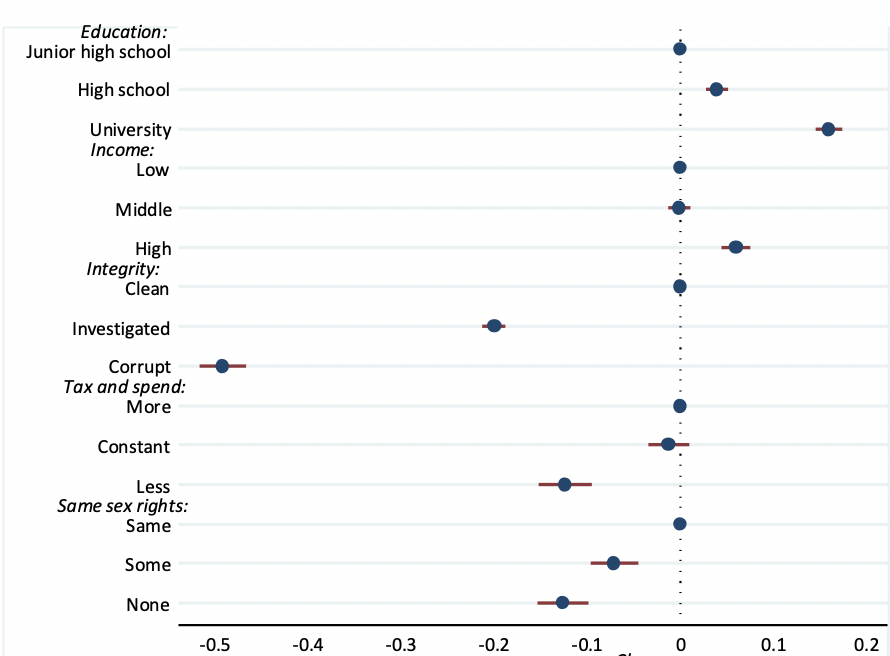
\includegraphics[scale = 0.6]{fz_conjoint.png}
\vspace{0.2cm}
\caption{\citet{franchino2015voting} conjoint: AMCE plot}
\small
\vspace{-0.3cm}
\label{fig: fz_amce}
\end{figure}

\end{frame}

%%%%%%%%%%%%%%%%%%%%%%%%%%%%%%%%%%%
\begin{frame}
\frametitle{Survey complexity and conjoint experiments}
\textcolor{Cerulean}{Proposal}: Compare the probability of voting for a candidate with outlier characteristics such as corruption to the probability of voting for a realistic candidate without this characteristic.
\begin{itemize}
\item E.g. What is the probability of a Democrat voting for a typical Democratic candidate?
\end{itemize}

\end{frame}


%%%%%%%%%%%%%%%%%%%%%%%%%%%%%%%%%%%
\begin{frame}
\frametitle{Survey complexity and conjoint experiments}

\begin{figure}[!hb]
\hspace*{-11mm}
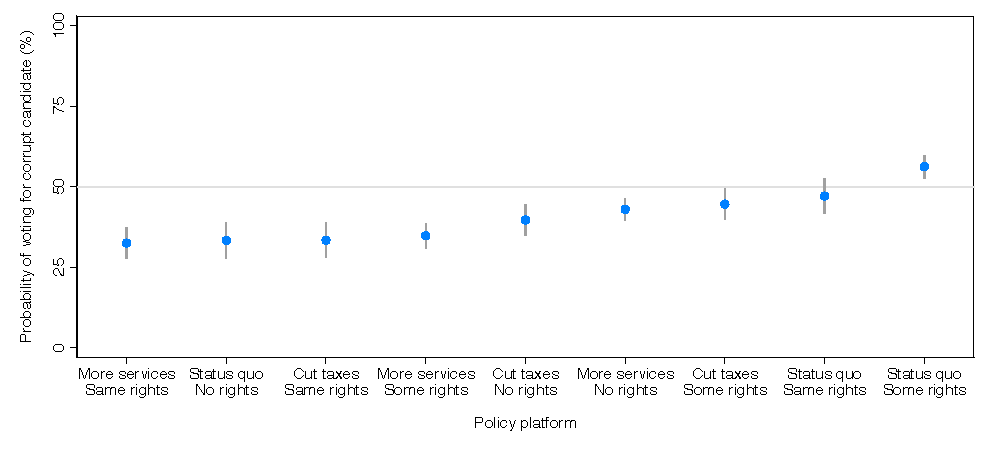
\includegraphics[scale = 0.77]{../figs/fz_margins_right.pdf}
\vspace{0.2cm}
\caption{\citet{franchino2015voting} conjoint: can policy positions overcome corruption (conservative respondents)?}
\small
\vspace{-0.3cm}
\label{fig: fz_margins_right}
\end{figure}

\end{frame}

%%%%%%%%%%%%%%%%%%%%%%%%%%%%%%%%%%%
\begin{frame}
\frametitle{Survey complexity and conjoint experiments}


\begin{figure}[!hb]
\hspace*{-11mm}
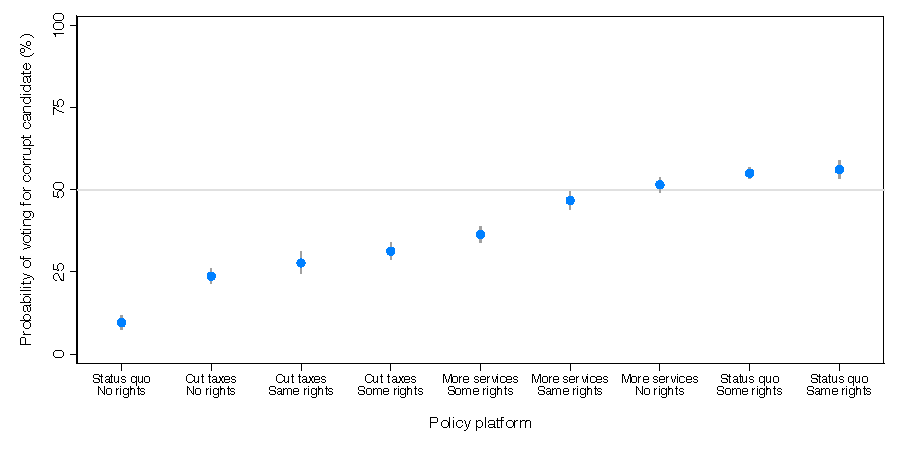
\includegraphics[scale = 0.77]{../figs/fz_margins_left.pdf}
\vspace{0.2cm}
\caption{\citet{franchino2015voting} conjoint: can policy positions overcome corruption (liberal respondents)?}
\small
\vspace{-0.5cm}
\label{fig: fz_margins_left}
\end{figure}

\end{frame}


%%%%%%%%%%%%%%%%%%%%%%%%%%%%%%%%%%%
\section{Conclusion}

\begin{frame}
\frametitle{Conclusion}
\begin{itemize}
\pause
\item Effect of corruption information on vote-choice \textcolor{Cerulean}{differs drastically} between field and survey experiments.
\begin{itemize}
\pause
\item \textcolor{Cerulean}{Zero} in field experiments.
\item \textcolor{Cerulean}{-33 to -35 percentage points} in survey experiments. 
\end{itemize}
\pause
\item Discrepancy does not seem to be driven by publication bias/p-hacking.
\pause
\item May arise from social desirability bias, lack of complexity and/or realism of hypothetical vignettes, and misinterpretation of results from conjoint experiments.

\end{itemize}
\end{frame}

%%%%%%%%%%%%%%%%%%%%%%%%%%%%%%%%%%%

\begin{frame}
\frametitle{Conclusion}
\begin{itemize}
\item Vote-choice survey experiments may provide information on the directionality of informational treatments, but point estimates they provide may not be representative of real-world voting behavior. 
\pause
\item Researchers should exercise caution when interpreting actions taken in hypothetical vignettes as indicative of real world behavior such as voting. 
\end{itemize}

\end{frame}



%%%%%%%%%%%%%%%%%%%%%%%%%%%%%%%%%%%

\bibliography{bibliography}
\end{document}